\chapter{Software Testing}Software testing is an investigation conducted to provide stakeholders with information about the quality of the product or service under test. Software testing can also provide an objective, independent view of the software to allow the business to appreciate and understand the risks of software implementation. Test techniques include, but are not limited to, the process of executing a program or application with the intent of finding software bugs (errors or other defects).


\section{Black Box Testing}

Black-box testing tests functional and non-functional characteristics of the software without referring to the internal code of the software. Redesigned the UI, to make the interface aesthetically good. Testing the routes, helped making it better to make routing simpler for ease of use.


\section{White Box Testing}

The proposed application contains various different modules and integrated successfully. Testing the algorithm which retrieves URL’s and Articles, kept timing out or didn’t scrape accurately. Modifying the algorithm by looping back to new URL if one didn’t exist helped run the scraper for longer time before being kicked out by the server itself.


\section{Unit Testing}

The unit testing is the process of testing the part of the program to verify whether the program is working correct or not. In this, the idea was to test if every route worked properly. The routing was redesigned. The homepage took longer to load when the stats were calculated live on server. Storing those time to time helped the server to respond faster.

\begin{figure}[htpb]
\centering
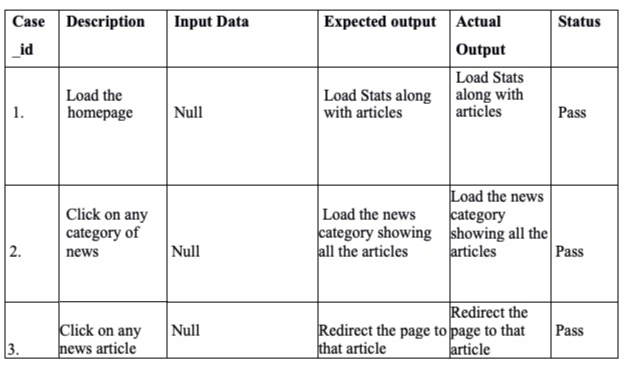
\includegraphics[width=\textwidth,height=\textheight,keepaspectratio]{../static/media/testCases.png}
\caption{Unit Testing}
\end{figure}


\section{Integration Testing}

Integration testing is also taken as integration and testing is the major testing process where the units are combined and tested. Its main objective is to verify whether the major parts of the program is working fine or not the application includes many and different constraints of functionalities and these modules are integrated and tested.

\begin{figure}[htpb]
\centering
\includegraphics[width=\textwidth,height=\textheight,keepaspectratio]{../static/media/\centering
\includegraphics[width=\textwidth,height=\textheight,keepaspectratio}
\caption{n{figure}[htpb}
\end{figure}[Integration Testing][itngTesting.png]
